\section{Xây dựng bộ thông dịch}
\label{ch3:interpreter}

    Sau khi đã đảm bảo câu lệnh đúng cú pháp thông qua bộ phân tích cú pháp (đã trình bày ở mục \textbf{\ref{ch3:syntax-analysis}}), thì việc cuối cùng cũng là việc quan trọng nhất của toàn bộ quá trình chính là thực thi câu lệnh, và việc này là phận sự của bộ thông dịch. Bộ thông dịch đóng vai trò to lớn nhất trong tất cả các bộ xử lý của trình thông dịch. Thiếu đi bộ thông dịch, trình thông dịch sẽ không bao giờ xử lý được chương trình. Hình dưới đây mô tả vị trí của bộ thông dịch trong toàn bộ cấu trúc của trình thông dịch Pandora:

\begin{figure}[H]
    \centering
    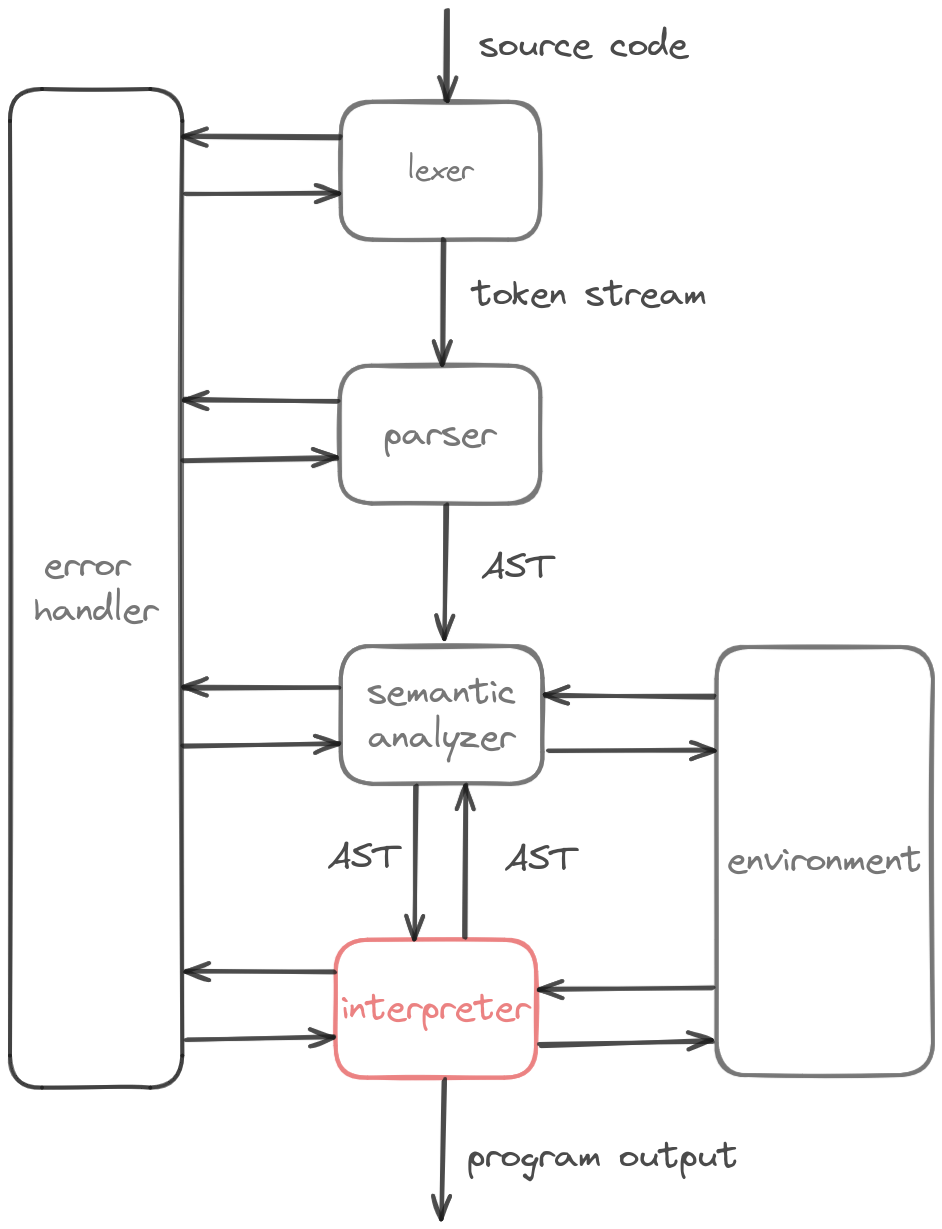
\includegraphics[scale=0.4]{interpreter-pos.png}
    \caption{Bộ thông dịch trong cấu trúc của trình thông dịch Pandora}
\end{figure}

    Đối với mỗi một câu lệnh hay một biểu thức, bộ thông dịch sẽ thực hiện \textbf{đánh giá} (evaluate) nó. Đánh giá một câu lệnh hay một biểu thức có thể được hiểu là thực hiện nó và trả về kết quả. Đánh giá một câu lệnh có thể là thực hiện các hành động như gán giá trị cho biến, thực hiện một hàm, v.v. Đánh giá một biểu thức có thể là tính toán giá trị của nó. Một biểu thức sau khi được đánh giá sẽ luôn trả về một giá trị. Ví dụ, biểu thức \kw{1 + 2} sẽ trả về giá trị \kw{3}. Một câu lệnh sau khi được đánh giá sẽ thường không trả về giá trị, nhưng nó có thể thay đổi trạng thái của chương trình. Ví dụ, câu lệnh \kw{a = 1} sẽ gán giá trị \kw{1} cho biến \kw{a}, nhưng nó không trả về giá trị nào cả; câu lệnh \kw{yeet 1;} sẽ ra khỏi hàm gọi nó, bỏ qua các câu lệnh còn lại trong hàm đó và trả về giá trị \kw{1}. 

    Để cho kiểu trả về của mỗi loại lệnh trở nên thống nhất, ta sẽ định nghĩa một kiểu dữ liệu mới là \kw{Value} để đại diện cho giá trị trả về của mỗi biểu thức. Kiểu dữ liệu này sẽ được định nghĩa trong tệp \kw{src/interpreter/eval.rs} như sau:

\begin{lstlisting}[]
pub struct Value {
    pub kind: ValueKind,
    pub span: Span,
}
\end{lstlisting}

    Trong đó, \kw{ValueKind} là một enum định nghĩa các loại giá trị mà một biểu thức có thể trả về, và \kw{Span} là một struct định nghĩa vị trí của một giá trị trong mã nguồn. \kw{ValueKind} sẽ được định nghĩa như sau:

\begin{lstlisting}[]
pub enum ValueKind {
    Int(i64),
    Float(f64),
    Str(String),
    Bool(bool),
    Function(Func),
    Char(char),
    Array(Vec<Value>),
    Unit,
}
\end{lstlisting}

    Trong đó, \kw{Int(i64)} đại diện cho một giá trị số nguyên, \kw{Float(f64)} đại diện cho một giá trị số thực, \kw{Str(String)} đại diện cho một giá trị chuỗi, \kw{Bool(bool)} đại diện cho một giá trị boolean, \kw{Function(Func)} đại diện cho một giá trị hàm (một biểu thức hàm sẵn sàng để đánh giá mỗi khi gọi hàm), \kw{Char(char)} đại diện cho một giá trị ký tự, \kw{Array(Vec<Value>)} đại diện cho một giá trị mảng, và \kw{Unit} đại diện cho một giá trị không có giá trị (đây là một giá trị đặc biệt của kiểu dữ liệu \kw{tuple}). 

    
    Còn đối với câu lệnh, ta sẽ định nghĩa một kiểu dữ liệu mới là \kw{StatementResult} để đại diện cho giá trị trả về của mỗi biểu thức. Kiểu dữ liệu này sẽ được định nghĩa trong tệp \kw{src/interpreter/eval.rs} như sau:

\begin{lstlisting}[]
StmtResult(Option<ControlFlow>),
\end{lstlisting}

    Trong đó, \kw{Option<ControlFlow>} đại diện cho việc một câu lệnh có thể trả về giá trị hoặc không trả về giá trị, còn \kw{ControlFlow} là một enum định nghĩa các loại giá trị mà một câu lệnh có thể trả về. \kw{ControlFlow} sẽ được định nghĩa như sau:

\begin{lstlisting}[]
pub enum ControlFlow {
    Continue,
    Break,
    Return(Value),
}
\end{lstlisting}

    Trong đó, \kw{Continue} đại diện cho việc tiếp tục thực thi câu lệnh tiếp theo, \kw{Break} đại diện cho việc thoát khỏi vòng lặp hiện tại, và \kw{Return(Value)} đại diện cho việc trả về giá trị \kw{Value} và thoát khỏi hàm hiện tại. Với cách xây dựng như vậy, ta đã đảm bảo rằng mọi câu lệnh đều có thể trả về giá trị, và mọi biểu thức đều có thể trả về giá trị.

\subsection{Đánh giá biểu thức (\textit{Expression evaluation})}

    Để thực hiện việc đánh giá một biểu thức, bộ thông dịch thông thường sẽ thực hiện một số công việc như sau:

\begin{itemize}
    \item \textbf{Kiểm tra kiểu dữ liệu}: Trước khi thực hiện một phép toán, bộ thông dịch sẽ kiểm tra xem kiểu dữ liệu của các toán hạng có phù hợp với phép toán đó không. Ví dụ, phép cộng chỉ có thể thực hiện giữa hai số nguyên hoặc hai số thực, không thể thực hiện giữa một số nguyên và một chuỗi. Bộ thông dịch làm điều này bằng cách cung cấp thông tin các toán hạng và phép toán cho bộ xử lý ngữ nghĩa, và bộ xử lý ngữ nghĩa sẽ kiểm tra xem phép toán đó có thể thực hiện được không (được phân tích ở mục \textbf{\ref{ch3:semantic-analysis}}).
    \item \textbf{Thực hiện phép toán}: Sau khi đã kiểm tra kiểu dữ liệu, bộ thông dịch sẽ thực hiện phép toán và trả về kết quả. Ví dụ, phép cộng giữa hai số nguyên \kw{1} và \kw{2} sẽ trả về giá trị \kw{3}.
\end{itemize}

    Bộ thông dịch sẽ thực hiện viiệc đánh giá một biểu thức bằng cách gọi một hàm \kw{interpret\_expr} trong tệp \kw{src/interpreter/expr.rs}. Hàm này sẽ nhận vào một biểu thức và trả về giá trị của nó. Để thực hiện việc này, ta sẽ định nghĩa hàm \kw{interpret\_expr} như sau:

\begin{lstlisting}[]
pub fn interpret_expr(
    env: &mut Environment,
    expr: &Box<Expr>,
    ...
) -> Result<Value, Vec<IError>> {
    ...
    let ty = match &expr.kind {
        ExprKind::Binary(...) => interpret_expr_binary(...)?,
        ExprKind::Identifier(...) => interpret_expr_ident(...)?,
        ExprKind::Literal(...) => interpret_expr_literal(...)?,
        ExprKind::FunCall(...) => interpret_expr_funcall(...)?,
        ExprKind::LibFunCall(...) => interpret_expr_lib_funcall(...)?,
        ExprKind::Cast(...) => interpret_expr_cast(...)?,
        ExprKind::Assign(...) => interpret_expr_assign(...)?,
        ExprKind::Unary(...) => interpret_expr_unary(...)?,
        ExprKind::AssignOp(...) => interpret_expr_assign_op(...)?,
        ExprKind::LibAccess(...) => interpret_expr_lib_access(...)?,
        ExprKind::Array(...) => interpret_expr_array(...)?,
        ExprKind::Index(...) => interpret_expr_index(...)?,
        ExprKind::Repeat(...) => interpret_expr_repeat(...)?,
    };
    ...
}
\end{lstlisting}

    Trong đó, \kw{env} kiểu \kw{Environment} đại diện cho môi trường hiện tại, \kw{expr} kiểu \kw{Box<Expr>} đại diện cho biểu thức cần đánh giá. Hàm này sẽ trả về một giá trị kiểu \kw{Value} hoặc một danh sách lỗi kiểu \kw{Vec<IError>}. Để thực hiện việc đánh giá một biểu thức, ta sẽ kiểm tra xem biểu thức đó thuộc loại nào và gọi hàm tương ứng. Ví dụ, nếu biểu thức là một biểu thức nhị phân, ta sẽ gọi hàm \kw{interpret\_expr\_binary} để đánh giá biểu thức đó.

    Do biểu thức trong ngôn ngữ Pandora rất đa dạng và phức tạp, ta sẽ chỉ trình bày cách thức đánh giá một số biểu thức cơ bản. 

\noindent \textbf{Đánh giá biểu thức nhị phân}

    Biểu thức nhị phân là một biểu thức mà có hai toán hạng và một toán tử. Ví dụ, biểu thức \kw{1 + 2} là một biểu thức nhị phân với toán hạng trái là \kw{1}, toán tử là \kw{+}, và toán hạng phải là \kw{2}. Để đánh giá một biểu thức nhị phân, ta cần đánh giá cả hai toán hạng và sau đó thực hiện phép toán. Để thực hiện việc này, ta sẽ định nghĩa một hàm \kw{interpret\_expr\_binary} trong tệp \kw{src/interpreter/expr.rs} như sau:

\begin{lstlisting}[]
fn interpret_expr_binary(
    env: &mut Environment,
    binop: &BinOp,
    lhs: &Box<Expr>,
    rhs: &Box<Expr>,
    ...
) -> Result<ValueKind, Vec<IError>> {
    ...
}
\end{lstlisting}

    Điều ta cần chú ý ở đây là tham số \kw{env} kiểu \kw{Environment} đại diện cho môi trường hiện tại, \kw{binop} kiểu \kw{BinOp} đại diện cho toán tử, \kw{lhs} kiểu \kw{Box<Expr>} đại diện cho toán hạng trái, \kw{rhs} kiểu \kw{Box<Expr>} đại diện cho toán hạng phải. Hàm này sẽ trả về một giá trị kiểu \kw{ValueKind} hoặc một danh sách lỗi kiểu \kw{Vec<IError>}.

    Việc đầu tiên ta cần thực hiện là đánh giá cả hai toán hạng. Để thực hiện việc này, ta sẽ gọi hàm \kw{interpret\_expr} đối với cả hai toán hạng:

\begin{lstlisting}[]
fn interpret_expr_binary(...) -> Result<ValueKind, Vec<IError>> {
    ...
    let lhs = interpret_expr(env, lhs, ...)?;
    let rhs = interpret_expr(env, rhs, ...)?;
    ...
}
\end{lstlisting}

    Hàm \kw{interpret\_expr} sẽ đánh giá một biểu thức và trả về giá trị của nó. Sau khi đã đánh giá cả hai toán hạng, ta sẽ tiến hành kiểm tra ngữ nghĩa của chúng. Chẳng hạn, nếu toán tử là \kw{+}, thì cả hai toán hạng đều phải là số nguyên hoặc số thực, còn nếu không thì ta sẽ trả về một lỗi. Sau khi đã kiểm tra ngữ nghĩa, ta sẽ thực hiện phép toán. Để thực hiện phép toán, ta sẽ kiểm tra xem toán tử là gì và thực hiện phép toán tương ứng. Đoạn mã sau mô tả cách thức thực hiện phép cộng:

\begin{lstlisting}[]
fn interpret_expr_binary(...) -> Result<ValueKind, Vec<IError>> {
    ...
    match &binop.node {
        ...
        BinOpKind::Add => match (lhs.kind, rhs.kind) {
            (ValueKind::Int(lhs), ValueKind::Int(rhs)) => Ok(ValueKind::Int(lhs + rhs)),
            (ValueKind::Float(lhs), ValueKind::Float(rhs)) => Ok(ValueKind::Float(lhs + rhs)),
            (ValueKind::Str(lhs), ValueKind::Str(rhs)) => {
                Ok(ValueKind::Str(format!("{}{}", lhs, rhs)))
            }
            _ => {
                return Err(vec![IError::CannotAdd {...}])
            }
        },
        ...
    }
    ...
}
\end{lstlisting}

    Trong đoạn mã trên, ta kiểm tra xem toán tử là \kw{+} hay không. Nếu là \kw{+}, ta kiểm tra xem cả hai toán hạng có phải là số nguyên hay số thực không. Nếu cả hai toán hạng đều là số nguyên, ta trả về giá trị là tổng của chúng, còn nếu cả hai toán hạng đều là số thực, ta trả về giá trị là tổng của chúng, còn nếu cả hai toán hạng đều là chuỗi, ta trả về giá trị là chuỗi kết hợp của chúng. Nếu không, ta trả về một lỗi. 

    Đoạn mã trên chỉ mô tả cách thức thực hiện phép cộng, còn các phép toán khác cũng sẽ được thực hiện tương tự.

\noindent \textbf{Đánh giá biểu thức hằng}

    Biểu thức hằng là một biểu thức mà không chứa bất kỳ biểu thức con nào. Ví dụ, biểu thức \kw{1} là một biểu thức hằng. Để đánh giá một biểu thức hằng, ta chỉ cần trả về giá trị của nó. Để thực hiện việc này, ta sẽ định nghĩa một hàm \kw{interpret\_expr\_literal} trong tệp \kw{src/interpreter/expr.rs} như sau:

\begin{lstlisting}[]
fn interpret_expr_literal(value: &Lit, span: Span) -> Result<ValueKind, Vec<IError>> {
    let Lit { kind, symbol } = value;
    let val = symbol.as_str();
    match kind {
        LitKind::Int => Ok(ValueKind::Int(parse_int_number(val, span)?)),
        LitKind::Float => Ok(ValueKind::Float(parse_float_number(val)?)),
        LitKind::Str => Ok(ValueKind::Str(parse_str(val))),
        LitKind::Bool => Ok(ValueKind::Bool(parse_bool(val))),
        LitKind::Char => Ok(ValueKind::Char(parse_char(val))),
        LitKind::RawStr(_) => Ok(ValueKind::Str(val.to_string())),
        LitKind::Err => unreachable!(),
    }
}
\end{lstlisting}

    Trong đó, \kw{value} kiểu \kw{Lit} đại diện cho biểu thức hằng, \kw{span} kiểu \kw{Span} đại diện cho vị trí của biểu thức hằng trong mã nguồn. Hàm này sẽ trả về một giá trị kiểu \kw{ValueKind} hoặc một danh sách lỗi kiểu \kw{Vec<IError>}. Để thực hiện việc này, ta sẽ kiểm tra xem biểu thức hằng đó là kiểu gì và trả về giá trị tương ứng. Ví dụ, nếu biểu thức hằng là một số nguyên, ta sẽ trả về giá trị số nguyên của nó, còn nếu biểu thức hằng là một số thực, ta sẽ trả về giá trị số thực của nó, v.v. Trong quá trình tính toán giá trị của một biểu thức hằng, ta cũng cần kiểm tra xem giá trị của biểu thức hằng đó có hợp lệ không. Ví dụ, nếu biểu thức hằng là một số nguyên, ta cần kiểm tra xem giá trị của nó có phải là một số nguyên hợp lệ không. Nếu không, ta sẽ trả về một lỗi. Chẳng hạn, nếu biểu thức hằng là một giá trị logic (boolean), ta cần kiểm tra xem giá trị của nó có phải là \kw{true} hoặc \kw{false} không. Nếu không, ta sẽ trả về một lỗi. Đoạn mã sau mô tả cách thức kiểm tra xem một giá trị có phải là một giá trị logic hợp lệ không:

\begin{lstlisting}[]
fn parse_bool(input: &str) -> bool {
    match kw::from_str(input) {
        Ok(keyword) => match keyword {
            Keyword::True => true,
            Keyword::False => false,
            _ => unreachable!(),
        },
        Err(_) => unreachable!(),
    }
}
\end{lstlisting}

\noindent \textbf{Đánh giá biểu thức gọi hàm}

    Biểu thức gọi hàm là một biểu thức mà có một hàm và một danh sách các tham số. Ví dụ, biểu thức \kw{f(1, 2)} là một biểu thức gọi hàm với hàm là \kw{f} và danh sách tham số là \kw{1} và \kw{2}. Để đánh giá một biểu thức gọi hàm, ta cần đánh giá hàm và tất cả các tham số, sau đó thực hiện hàm với các tham số đó. Để thực hiện việc này, ta sẽ định nghĩa một hàm \kw{interpret\_expr\_funcall} trong tệp \kw{src/interpreter/expr.rs} như sau:

\begin{lstlisting}[]
fn interpret_expr_funcall(
    env: &mut Environment,
    prefix: &Box<Expr>,
    args: &Vec<Box<Expr>>,
    ...
) -> Result<ValueKind, Vec<IError>> {
    ...
}
\end{lstlisting}

    Trong đó, \kw{env} kiểu \kw{Environment} đại diện cho môi trường hiện tại, \kw{prefix} kiểu \kw{Box<Expr>} đại diện cho hàm, \kw{args} kiểu \kw{Vec<Box<Expr>>} đại diện cho danh sách tham số. Hàm này sẽ trả về một giá trị kiểu \kw{ValueKind} hoặc một danh sách lỗi kiểu \kw{Vec<IError>}. Để thực hiện việc này, trước tiên, ta cần kiểm tra xem \kw{prefix} có phải là một tên hàm hợp lệ không. Nếu không, ta sẽ trả về một lỗi. Đoạn mã sau mô tả cách thức kiểm tra xem một tên hàm có phải là một tên hàm hợp lệ không:

\begin{lstlisting}[]
fn interpret_expr_funcall(...) -> Result<ValueKind, Vec<IError>> {
    let ident = match &prefix.kind {
        ExprKind::Identifier(ident) => ident,
        _ => return Err(vec![IError::InvalidFunctionCall {...}]),
    };
    ...
}
\end{lstlisting}

Sau khi đã kiểm tra xem \kw{prefix} có phải là một tên hàm hợp lệ không, ta sẽ kiểm tra xem hàm đó có tồn tại trong môi trường hiện tại không. Nếu không, ta sẽ kiểm tra xem hàm đó có tồn tại trong thư viện chuẩn không. Nếu có, ta sẽ cần đánh giá tất cả các tham số và thực hiện hàm đó với các tham số đó. Do các tham số đều là biểu thức, ta có thể lần lượt đánh giá từng tham số bằng cách gọi hàm \kw{interpret\_expr} đối với từng tham số. Sau khi đã đánh giá tất cả các tham số, ta sẽ thực hiện kiểm tra ngữ nghĩa của chúng và thực hiện hàm đó với các tham số trên:

\begin{lstlisting}[]
fn interpret_expr_funcall(...) -> Result<ValueKind, Vec<IError>> {
    ...
    let result = env.lookup_function(ident.name.as_str());
    let evaluated_args = {
        let mut args_vec = Vec::new();
        for arg in args {
            args_vec.push((interpret_expr(env, arg, ...)?, ...));
        }
        args_vec
    };

    if result.is_none() {
        // We will try to find the function in the standard library
        ...
        if let Some(lib) = env.lookup_default_library("std") {
            if let Some(func) = lib.get_function(std_func_name) {
                ...
                return func(..., evaluated_args);
            } else {
                return Err(vec![IError::FunctionNotInScope {...}]);
            }
        } else {
            unreachable!("Standard library must be loaded");
        }
    }
    ...
}
\end{lstlisting}

    Trong đoạn mã trên, có một điểm cần lưu ý. Mặc dù, trên lý thuyết, ta sẽ kiểm tra xem hàm đó có tồn tại trong thư viện chuẩn không trước khi thực hiện đánh giá tất cả các tham số, nhưng thực tế, ta sẽ thực hiện đánh giá tất cả các tham số trước, sau đó mới kiểm tra xem hàm đó có tồn tại trong thư viện chuẩn không. Điều này là do cơ chế borrowing trong Rust. Khi ta đánh giá một tham số, ta sẽ cần truy cập đến môi trường hiện tại, và khi ta kiểm tra xem hàm đó có tồn tại trong thư viện chuẩn không, ta cũng sẽ cần truy cập đến môi trường hiện tại. Tuy nhiên, một môi trường chỉ có thể được truy cập một lần tại một thời điểm, nếu ta đã truy cập môi trường hiện tại để đánh giá một tham số, ta sẽ không thể truy cập môi trường hiện tại để kiểm tra xem hàm đó có tồn tại trong thư viện chuẩn không. Để giải quyết vấn đề này, ta sẽ thực hiện đánh giá tất cả các tham số trước, sau đó mới kiểm tra xem hàm đó có tồn tại trong thư viện chuẩn không. Điều này sẽ đảm bảo rằng ta chỉ truy cập môi trường hiện tại một lần tại một thời điểm và tránh được lỗi borrowing.

    Nếu hàm đó tồn tại trong môi trường hiện tại, ta sẽ thực hiện hàm đó với các tham số trên thông qua hàm \kw{Value::evaluate\_function}:

\begin{lstlisting}[]
fn interpret_expr_funcall(...) -> Result<ValueKind, Vec<IError>> {
    ...
    let result = env.lookup_function(ident.name.as_str());
    let evaluated_args = {
        let mut args_vec = Vec::new();
        for arg in args {
            args_vec.push((interpret_expr(env, arg, ...)?, ...));
        }
        args_vec
    };
    ...

    Value::evaluate_function(
        env,
        result.unwrap().1,
        evaluated_args,
        ...
    )
}
\end{lstlisting}

    Trong đó, \kw{env} kiểu \kw{Environment} đại diện cho môi trường hiện tại, \kw{result.unwrap().1} đại diện cho hàm cần thực hiện, \kw{evaluated\_args} đại diện cho danh sách tham số. Hàm \kw{Value::evaluate\_function} sẽ thực hiện hàm đó với các tham số trên và trả về giá trị của hàm đó:

\begin{lstlisting}[]
pub fn evaluate_function(
    env: &Environment,
    function: ValueKind,
    evaluated_args: Vec<(Value, bool)>,
    ...
) -> Result<ValueKind, Vec<IError>> {
    ...
    match function {
        ValueKind::Function(func) => {
            let Func { sig, body } = func;

            // create a new environment for the function
            let mut func_env = Environment::new_with_parent(env, ...);
            func_env.in_function = true;

            // semantic analysis
            ...

            let result = stmt::interpret_stmt(&mut func_env, &body, ...)?;

            // handle return value
            match result {
                EvalResult::StmtResult(control_flow) => match control_flow {
                    Some(ControlFlow::Return(val)) => {
                        // semantic analysis
                        ...
                        
                        if errors.is_empty() {
                            Ok(val.kind)
                        } else {
                            Err(errors)
                        }
                    }
                    None => {
                        // semantic analysis
                        ...
                        if errors.is_empty() {
                            Ok(ValueKind::Unit)
                        } else {
                            Err(errors)
                        }
                    }
                    _ => unreachable!("function body should not return continue or break"),
                },
            }

        },
        _ => unreachable!("This should be a function"),
    }
    ...
}
\end{lstlisting}

    Đoạn mã trên mô tả cách thức thực hiện hàm. Đầu tiên, ta sẽ tạo một môi trường mới cho hàm đó và thực hiện hàm đó trong môi trường mới vừa tạo. Trước khi thực hiện hàm, ta cũng cần thực hiện kiểm tra ngữ nghĩa của hàm đó. Sau khi đảm bảo tính đúng đắn về ngữ nghĩa, ta sẽ thực hiện hàm thông qua việc đánh giá câu lệnh của hàm đó bằng cách gọi hàm \kw{stmt::interpret\_stmt} (sẽ được phân tích sau). Sau khi đã thực hiện hàm, ta sẽ kiểm tra xem hàm đó có trả về giá trị không. Nếu có, ta sẽ trả về giá trị đó, còn nếu không, ta sẽ trả về giá trị \kw{Unit}. 

\subsection{Đánh giá câu lệnh (\textit{Statement evaluation})}

    Để thực hiện đánh giá một câu lệnh, ta sẽ gọi một hàm \kw{interpret\_stmt} trong tệp \kw{src/interpreter/stmt.rs}. Hàm này sẽ nhận vào một câu lệnh và trả về giá trị của nó. Để thực hiện việc này, ta sẽ định nghĩa hàm \kw{interpret\_stmt} như sau:

\begin{lstlisting}[]
pub fn interpret_stmt(
    env: &mut Environment,
    stmt: &Box<Stmt>,
    ...
) -> IResult {
    ...
    match &stmt.kind {
        StmtKind::Import(...) => interpret_stmt_import(...),
        StmtKind::Expr(...) => interpret_stmt_expr(...),
        StmtKind::Var(...) => interpret_stmt_var_decl(...),
        StmtKind::If(...) => interpret_stmt_if(...),
        StmtKind::While(...) => interpret_stmt_while(...),
        StmtKind::Break => interpret_stmt_break(...),
        StmtKind::Continue => interpret_stmt_continue(...),
        StmtKind::Block(...) => interpret_stmt_block(...),
        StmtKind::FuncDecl(...) => interpret_stmt_func_decl(...),
        StmtKind::Return(...) => interpret_stmt_return(...),
        StmtKind::For(...) => interpret_stmt_for(...),
        StmtKind::Empty => Ok(EvalResult::StmtResult(...)),
    }
}
\end{lstlisting}

    Trong đó, \kw{env} kiểu \kw{Environment} đại diện cho môi trường hiện tại, \kw{stmt} kiểu \kw{Box<Stmt>} đại diện cho câu lệnh cần đánh giá. Hàm này sẽ trả về một giá trị kiểu \kw{IResult}. \kw{IResult} là một \textit{alias} cho kiểu dữ liệu \kw{Result<EvalResult} \kw{, Vec<IError>}\kw{>}, đại diện cho kết quả của việc đánh giá một câu lệnh. 

    \kw{EvalResult} là một enum định nghĩa các loại giá trị có thể trả về sau khi đánh giá một câu lệnh hay một biểu thức. \kw{IError} là một struct định nghĩa một lỗi trong quá trình đánh giá một câu lệnh hay một biểu thức. Ta sẽ định nghĩa các đối tượng kể trên như sau:

\begin{lstlisting}[]
pub type IResult = Result<EvalResult, Vec<IError>>;

pub enum EvalResult {
    StmtResult(Option<ControlFlow>),
    ...
}

pub enum IError {
    ...
}
\end{lstlisting}

    Để thực hiện việc này, ta sẽ kiểm tra xem câu lệnh đó thuộc loại nào và gọi hàm tương ứng. Ví dụ, nếu câu lệnh là một câu lệnh gán, ta sẽ gọi hàm \kw{interpret\_stmt\_assign} để đánh giá câu lệnh đó.

    Tương tự như việc đánh giá biểu thức, ta sẽ chỉ trình bày cách thức đánh giá một số câu lệnh cơ bản.

\noindent \textbf{Đánh giá câu lệnh khai báo biến}

    Câu lệnh khai báo biến là một câu lệnh mà khai báo một biến mới. Ví dụ, câu lệnh \kw{set x: int = 1;} là một câu lệnh khai báo biến với tên biến là \kw{x} và giá trị là \kw{1}. Đoạn mã sau mô tả cách thức đánh giá một câu lệnh khai báo biến:

\begin{lstlisting}[]
pub fn interpret_stmt_var_decl(
    env: &mut Environment,
    local: &Local,
    ...
) -> IResult {
    ...
    let Local {
        is_mut,
        ident,
        ty,
        kind,
        ...
    } = local;

    let decl_ty = interpret_ty(env, ty, ...)?;

    // If the variable is array, it must have a length if it is not declared with an initializer
    let (value, var_ty_kind, ...) = match kind {
        LocalKind::Init(expr) => {
            let value = interpret_expr(env, expr, ...)?;

            // semantic analysis
            ...
        }
        LocalKind::Decl => ...,
    };

    let decl_ty = Ty {
        kind: var_ty_kind,
        ...
    };
    let ident = Ident {
        name: ident.name.to_string(),
        ...
    };
    env.insert_variable(ident, value, *is_mut, decl_ty, ...);
    Ok(EvalResult::StmtResult(None))
}
\end{lstlisting}

    Trong đoạn mã trên, \kw{env} kiểu \kw{Environment} đại diện cho môi trường hiện tại, \kw{local} kiểu \kw{Local} đại diện cho câu lệnh khai báo biến. Hàm này sẽ trả về một giá trị kiểu \kw{IResult}. Đầu tiên, ta sẽ kiểm tra kiểu dữ liệu của biến thông qua hàm \kw{interpret\_ty}. Sau đó, ta sẽ kiểm tra xem biến đó có được khởi tạo hay không. Nếu có, ta sẽ đánh giá giá trị của biến thông qua hàm \kw{interpret\_expr} và thực hiện kiểm tra ngữ nghĩa của nó. Sau khi đã đánh giá giá trị của biến, ta sẽ thêm biến đó vào môi trường hiện tại thông qua hàm \kw{env.insert\_variable}. Câu lệnh khai báo biến sẽ không trả về giá trị nên ta sẽ trả về \kw{None}.

\noindent \textbf{Đánh giá câu lệnh biểu thức}

    Câu lệnh biểu thức là một câu lệnh mà chỉ chứa một biểu thức. Ví dụ, câu lệnh \kw{1 + 2;} là một câu lệnh biểu thức. Đoạn mã sau mô tả cách thức đánh giá một câu lệnh biểu thức:

\begin{lstlisting}[]
pub fn interpret_stmt_expr(
    env: &mut Environment,
    expr: &Box<Expr>,
    ...
) -> IResult {
    ...
    interpret_expr(env, expr, ...)?;
    Ok(EvalResult::StmtResult(None))
}
\end{lstlisting}

    Trong đoạn mã trên, \kw{env} kiểu \kw{Environment} đại diện cho môi trường hiện tại, \kw{expr} kiểu \kw{Box<Expr>} đại diện cho biểu thức. Hàm này sẽ trả về một giá trị kiểu \kw{IResult}. Để thực hiện việc này, ta sẽ gọi hàm \kw{interpret\_expr} để đánh giá biểu thức và trả về giá trị của nó (chi tiết hàm đã được phân tích phía trên). Tương tự với câu lệnh khai báo biến, câu lệnh này cũng không trả về giá trị nên ta sẽ trả về \kw{None}.

\noindent \textbf{Đánh giá câu lệnh trả về}

Câu lệnh trả về là một câu lệnh thoát khỏi hàm và trả về một giá trị. Những câu lệnh sau câu lệnh này trong hàm đó sẽ không được thực thi. Ví dụ, câu lệnh \kw{yeet 3;} sẽ kết thúc hàm hiện tại đang xét và trả về giá trị \kw{3}. Đoạn mã sau sẽ mô tả cách thức đánh giá một câu lệnh trả về:

\begin{lstlisting}[]
pub fn interpret_stmt_return(
    env: &mut Environment,
    expr: &Option<Box<Expr>>,
    ...
) -> IResult {
    ...

    let value = match expr {
        Some(expr) => interpret_expr(env, expr, ...)?,
        None => Value {
            kind: ValueKind::Unit,
            ...
        },
    };
    Ok(EvalResult::StmtResult(Some(ControlFlow::Return(value))))
}
\end{lstlisting}

    Ở đoạn mã trên, \kw{env} kiểu \kw{Environment} đại diện cho môi trường hiện tại, kiểu \kw{Option<Box<Expr>>} đại diện cho giá trị trả về. Hàm này sẽ trả về một giá trị kiểu \kw{IResult}. Đầu tiên, ta sẽ kiểm tra xem câu lệnh trả về có giá trị trả về hay không. Nếu có, ta sẽ đánh giá giá trị trả về thông qua hàm \kw{interpret\_expr}. Sau đó, ta sẽ trả về giá trị trả về thông qua \kw{ControlFlow::Return}. 

\noindent \textbf{Đánh giá câu lệnh rẽ nhánh}

Câu lệnh rẽ nhánh là một câu lệnh mà thực hiện một số câu lệnh dựa trên một điều kiện. Ví dụ, câu lệnh \kw{when x>5 \{println("x is greater than 5");\} alt \{println("x is not greater than 5");\}} là một câu lệnh rẽ nhánh. Đoạn mã sau mô tả cách thức đánh giá một câu lệnh rẽ nhánh:

\begin{lstlisting}[]
pub fn interpret_stmt_if(
    env: &mut Environment,
    cond: &Box<Expr>,
    then_block: &Box<Stmt>,
    else_block: &Option<Box<Stmt>>,
    ...
) -> IResult {
    ...
    let cond_result = interpret_expr(env, cond, in_loop, is_verbose);

    // semantic analysis
    ...

    let cond = cond_result.clone().unwrap();
    let is_true = match cond.kind {
        ValueKind::Bool(bool) => bool,
        _ => {
            return Err(vec![IError::MismatchedType {...}])
        }
    };

    if is_true {
        interpret_stmt(env, then_block, ...)
    } else {
        match else_block {
            Some(else_block) => interpret_stmt(env, else_block, ...),
            None => Ok(EvalResult::StmtResult(None)),
        }
    }
}
\end{lstlisting}

    Trong đoạn mã trên, \kw{env} kiểu \kw{Environment} đại diện cho môi trường hiện tại, \kw{cond} kiểu \kw{Box<Expr>} đại diện cho điều kiện, \kw{then\_block} kiểu \kw{Box<Stmt>} đại diện cho khối lệnh thực thi nếu điều kiện đúng, \kw{else\_block} kiểu \kw{Option<Box<Stmt>}\kw{>} đại diện cho khối lệnh thực thi nếu điều kiện sai. Hàm này sẽ trả về một giá trị kiểu \kw{IResult}. Đầu tiên, ta sẽ đánh giá điều kiện thông qua hàm \kw{interpret\_expr}. Sau đó, ta sẽ kiểm tra xem điều kiện đó có phải là một giá trị logic hay không. Nếu không, ta sẽ trả về một lỗi. Sau khi đã kiểm tra điều kiện, ta sẽ thực hiện khối lệnh thích hợp dựa trên giá trị của điều kiện. Nếu điều kiện đúng, ta sẽ thực hiện khối lệnh \kw{then\_block}, còn nếu điều kiện sai, ta sẽ thực hiện khối lệnh \kw{else\_block} nếu có.
